%%%%%%%%%%%%%%%%%%%%%%
%ndss and S&P
%\documentclass[conference]{IEEEtran}
%\pagestyle{plain}

%CCS
\documentclass[sigconf, anonymous]{acmart}
\fancyhf{} % Remove fancy page headers 
\fancyhead[C]{Anonymous submission \#9999 to ACM CCS 2021} % TODO: replace 9999 with your paper number
\fancyfoot[C]{\thepage}

\setcopyright{none} % No copyright notice required for submissions
\acmConference[Anonymous Submission to ACM CCS 2021]{ACM Conference on Computer and Communications Security}{Due 15 May 2019}{London, TBD}
\acmYear{2021}
\settopmatter{printacmref=false, printccs=true, printfolios=true} % We want page numbers on submissions


%%%%%%%%%%%%%%%%%%%%%%
% \usepackage{enumitem}
\usepackage{graphicx}
\usepackage{xcolor}
\usepackage{pifont}
% \usepackage[draft]{hyperref}
\usepackage{adjustbox}
\usepackage{caption}
\usepackage{subcaption}
\usepackage{mathtools}
\usepackage{mathrsfs}
\usepackage{xspace}
\usepackage{url}
\usepackage[mode=buildnew]{standalone}
\usepackage{tikz}
\usepackage{pifont}
\usepackage{wasysym}
\usepackage{booktabs}
\usepackage{multirow}
\usetikzlibrary{positioning, trees, arrows, calc, automata}
% \usepackage{enumitem}
\usepackage{cleveref}
\usepackage{mfirstuc}
\usepackage{pifont}
%\usepackage[font={small}]{caption}
%\usepackage{enumitem}
%\usepackage[shortlabels]{enumitem}
%\usepackage{cite}
%\usepackage{flushend}
%\usepackage{hyperref}
%\usepackage{caption}

% \usepackage[
% all=normal%
% ,floats=tight%
% ,paragraphs=tight%
% % ,wordspacing=tight
% %,mathspacing=tight
% %,mathdisplays=tight
% ]{savetrees}

%\hypersetup{draft}

%% tikz figure icon definitions
% \pgfdeclareimage[width=2cm]{enclave}{icons/enclave}
% \pgfdeclareimage[width=2cm]{enclave-yellow}{icons/sgx_red}
% \pgfdeclareimage[width=2cm]{enclave-red}{icons/sgx_yellow}
% \pgfdeclareimage[width=2cm]{server}{icons/server_contoured}
% \pgfdeclareimage[width=2cm]{blockchain}{icons/blockchain}
% \pgfdeclareimage[width=2cm]{user}{icons/persons/user/user}
% \pgfdeclareimage[width=2cm]{attacker}{icons/persons/burglar}
% \pgfdeclareimage[width=1cm]{phone}{icons/smartphone}
% \pgfdeclareimage[width=2cm]{computer}{icons/devices/client}

% \pgfdeclareimage[width=2cm]{memory}{icons/computerpack/013-ram}
% \pgfdeclareimage[width=1.4cm]{gpu}{icons/computerpack/002-vga}
% \pgfdeclareimage[width=1.4cm]{mouse}{icons/computerpack/017-mouse}
% \pgfdeclareimage[width=1.4cm]{keyboard}{icons/computerpack/024-keyboard}
% \pgfdeclareimage[width=1.4cm]{screen}{icons/computerpack/018-monitor-2}
% \pgfdeclareimage[width=1.4cm]{lan}{icons/computerpack/023-lan}
% \pgfdeclareimage[width=1.4cm]{lanred}{icons/computerpack/023-lan-red}

% \definecolor{col1}{RGB}{170, 72, 59}
% \definecolor{col2}{RGB}{170,114, 59}
% \definecolor{col3}{RGB}{ 38, 93,105}
% \definecolor{col4}{RGB}{ 44,127, 66}

\definecolor{col1}{HTML}{4398D1}
\definecolor{col2}{HTML}{FF4842}
\definecolor{col3}{RGB}{ 38, 93,105}
\definecolor{col4}{RGB}{ 44,127, 66}

\definecolor{greenc}{HTML}{64c37d}
\definecolor{redc}{HTML}{e13957}

\ifstandalone
    \newcommand{\icon}[1]{../icons/#1}
\else
    \newcommand{\icon}[1]{images/icons/#1}
\fi

\newcommand{\imgmemory}{
\includegraphics[width=2.0cm]{\icon{computerpack/013-ram}}}
\newcommand{\imggpu}{
\includegraphics[width=1.4cm]{\icon{computerpack/002-vga}}}
\newcommand{\imggpusmall}{
\includegraphics[width=1.0cm]{\icon{computerpack/002-vga}}}
\newcommand{\imgmouse}{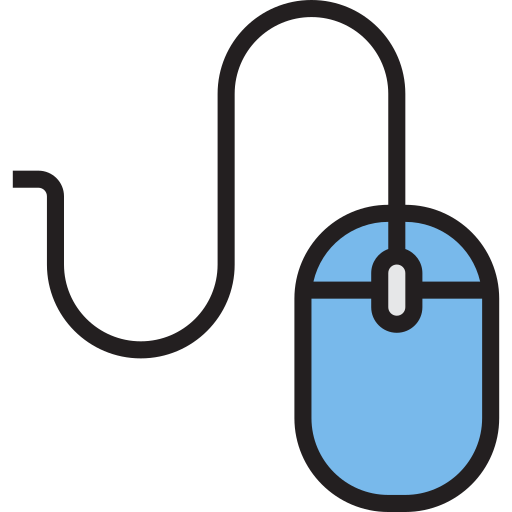
\includegraphics[width=1.4cm]{\icon{computerpack/017-mouse}}}
\newcommand{\imgkeyboard}{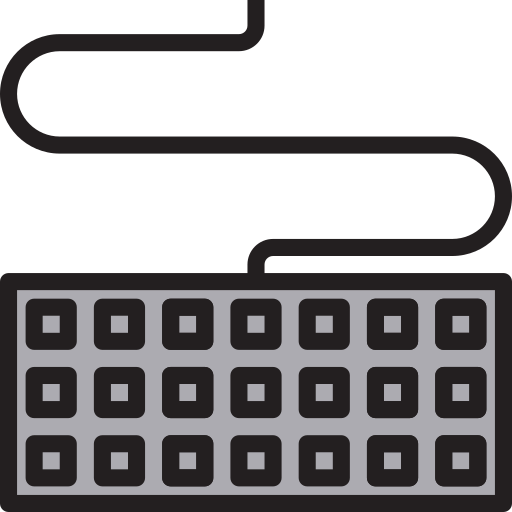
\includegraphics[width=1.4cm]{\icon{computerpack/024-keyboard}}}
\newcommand{\imgscreen}{\includegraphics[width=1.4cm]{\icon{computerpack/018-monitor}}}
\newcommand{\imglan}{
\includegraphics[width=1.4cm]{\icon{computerpack/023-lan}}}
\newcommand{\imglanred}{
\includegraphics[width=1.4cm]{\icon{computerpack/023-lan-red}}}
\newcommand{\imgcpu}{
\includegraphics[width=1.4cm]{\icon{computerpack/034-cpu}}}
\newcommand{\imgcpusmall}{
\includegraphics[width=1.0cm]{\icon{computerpack/034-cpu}}}

\newcommand{\imgdisplay}{\includegraphics[height=1.4cm]{\icon{computerpack/021-mobile}}}
\newcommand{\imgdisplaysmall}{\includegraphics[height=1.0cm]{\icon{computerpack/021-mobile}}}
\newcommand{\imgsim}{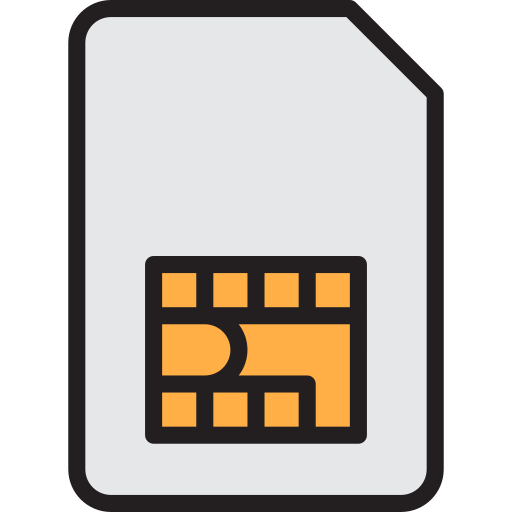
\includegraphics[height=1.4cm]{\icon{computerpack/008-sim-card}}}
\newcommand{\imgsimsmall}{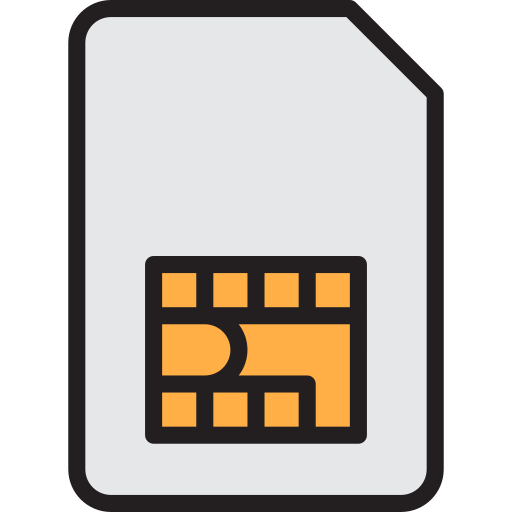
\includegraphics[height=1.0cm]{\icon{computerpack/008-sim-card}}}
\newcommand{\imgsd}{
\includegraphics[height=1.4cm]{\icon{computerpack/011-sd-card}}}
\newcommand{\imgsdsmall}{
\includegraphics[height=1.0cm]{\icon{computerpack/011-sd-card}}}
\newcommand{\imgcamera}{\includegraphics[width=1.4cm]{\icon{computerpack/035-camera}}}
\newcommand{\imgcamerasmall}{\includegraphics[width=1.0cm]{\icon{computerpack/035-camera}}}

\newcommand{\imgenclave}{\includegraphics[width=2.0cm]{\icon{enclave}}}
\newcommand{\imgenclavesmall}{\includegraphics[width=1.4cm]{\icon{enclave}}}
\newcommand{\imgenclavesmaller}{\includegraphics[width=1.0cm]{\icon{enclave}}}
\newcommand{\imgenenclavered}{\includegraphics[width=2.0cm]{\icon{sgx_red}}}
\newcommand{\imgenenclaveredsmall}{\includegraphics[width=1.0cm]{\icon{sgx_red}}}
\newcommand{\imguser}{
\includegraphics[height=2.0cm]{\icon{persons/user/user}}}
\newcommand{\imgusersmall}{
\includegraphics[height=1.4cm]{\icon{persons/user/user}}}
\newcommand{\imgattacker}{
\includegraphics[width=2.0cm]{\icon{persons/burglar}}}
\newcommand{\imgattackersmall}{
\includegraphics[height=1.4cm]{\icon{persons/burglar}}}
\newcommand{\imgcomputer}{
\includegraphics[width=2.0cm]{\icon{devices/client}}}

\newcommand{\imglock}{\includegraphics[width=0.3cm]{\icon{lock-icon}}}
\newcommand{\imglocklarge}{\includegraphics[width=0.5cm]{\icon{lock-icon}}}
\newcommand{\imgkeyyellow}{\includegraphics[width=0.5cm]{\icon{key-yellow}}}
\newcommand{\imgkeyred}{\includegraphics[width=0.5cm]{\icon{key-red}}}
\newcommand{\imgkeyblue}{\includegraphics[width=0.5cm]{\icon{key-blue}}}
\newcommand{\imgcertred}{\includegraphics[width=0.5cm]{\icon{certificate-red}}}
\newcommand{\imgcertyellow}{\includegraphics[width=0.5cm]{\icon{certificate-yellow}}}
\newcommand{\imgcertblue}{\includegraphics[width=0.5cm]{\icon{certificate-blue}}}

\newcommand{\imgdevil}{\includegraphics[width=0.6cm]{\icon{devil}}}

\let\oldding\ding% Store old \ding in \oldding
\renewcommand{\ding}[2][1]{\scalebox{#1}{\oldding{#2}}}% Scale \oldding via optional argument

\newcommand{\zero}{\ding[1.2]{171}\xspace}
\newcommand{\one}{\ding[1.2]{172}\xspace}
\newcommand{\two}{\ding[1.2]{173}\xspace}
\newcommand{\three}{\ding[1.2]{174}\xspace}
\newcommand{\four}{\ding[1.2]{175}\xspace}
\newcommand{\five}{\ding[1.2]{176}\xspace}
\newcommand{\six}{\ding[1.2]{177}\xspace}
\newcommand{\seven}{\ding[1.2]{178}\xspace}
\newcommand{\eight}{\ding[1.2]{179}\xspace}
\newcommand{\nine}{\ding[1.2]{180}\xspace}
\newcommand{\ten}{\ding[1.2]{181}\xspace}

\newcommand{\risc}{RISC-V\xspace}
\newcommand{\ce}{controller enclave\xspace}
\newcommand{\ces}{controller enclave\xspace}
\newcommand{\Ce}{Controller enclave\xspace}
\newcommand{\Ces}{Controller enclave\xspace}
\newcommand{\app}{application enclave\xspace}
\newcommand{\App}{Application enclave\xspace}
\newcommand{\apps}{application enclaves\xspace}
\newcommand{\Apps}{Application enclaves\xspace}


\newcommand*\circled[1]{\tikz[baseline= (char.base)]{
            \node[shape=circle,draw,inner sep=0.3pt] (char) {\(#1\)};}}

\newcommand{\blue}[1]{\textcolor{black}{#1}}
\newcommand{\red}[1]{\textcolor{red}{#1}}


\newcommand{\figsaver}[0]{\vspace{-5pt}}
\newcommand{\parasaver}[0]{\vspace{-2pt}}

\newif\ifremoveall{}
\removealltrue{}

\ifremoveall{}
\newcommand{\aritra}[1]{\textbf{\emph{ #1 \colorbox{green}{[Aritra]}}}}
\newcommand{\ip}[1]{\textbf{\emph{ #1 \colorbox{cyan}{[Ivan]}}}}
\newcommand{\moritz}[1]{\textbf{\emph{ #1 \colorbox{yellow}{[Moritz]}}}}
\newcommand{\srdjan}[1]{\textbf{\emph{ #1 \colorbox{blue}{[Srdjan]}}}}
\newcommand{\todo}[1]{\textcolor{red}{TODO: \@#1}}
\newcommand{\todoref}{\textcolor{red}{[ref]}}
\newcommand{\citneed}{[\textcolor{red}{cit}] }
\else
\newcommand{\aritra}[1]{}
\newcommand{\ip}[1]{}
\newcommand{\moritz}[1]{}
\newcommand{\todo}[1]{}
\newcommand{\todoref}[1]{}
\newcommand{\citneed}[1]{}
\fi


\newcommand{\name}{\textsc{PIE}\xspace}
\newcommand{\tool}{\textsc{\name{} API}\xspace}
\newcommand{\device}{\textsc{Device}\xspace}

\newcommand{\usb}{\texttt{USB}\xspace}
\newcommand{\tls}{\texttt{TLS}\xspace}

\def\nameenclave{platform-wide enclave\xspace}
\def\Nameenclave{Platform-wide enclave\xspace}

\newcommand{\sphw}[0]{specialized hardware\xspace}
\newcommand{\Sphw}[0]{Specialized hardware\xspace}


%%%%%%%%%%%%%%%%%%%%%%
%savetrees
\usepackage[
all=normal,floats=tight
,paragraphs=tight
% ,wordspacing=tight
,mathspacing=tight
% ,mathdisplays=tight
]{savetrees}
%%%%%%%%%%%%%%%%%%%%%%

% \newcommand{\myparagraph}[1]{\par\emph{#1.}\xspace}
\newcommand{\myparagraph}[1]{\paragraph{#1}}

\newcounter{para}
% \newcommand{\mypara}[1]{\refstepcounter{para}\emph{\thepara}.\space\emph{#1}.\xspace}
\newcommand{\mypara}[1]{\refstepcounter{para}\paragraph{\thepara.\space{}#1}}
% \newcommand{\mypara}[1]{\paragraph{#1}}
%\newcommand\mypara{\par\refstepcounter{para}\thepara\space}

%------------------------------------------------------------------------------
%                                Space savers.
%------------------------------------------------------------------------------
% This mylist environment indents items, and saves less space than the above.
\newcounter{myctr}
\newenvironment{mylist}{\begin{list}{\arabic{myctr}.}
{\usecounter{myctr}
\setlength{\topsep}{1mm}\setlength{\itemsep}{0.5mm}
\setlength{\parsep}{0.5mm}
\setlength{\itemindent}{1mm}\setlength{\partopsep}{0mm}
\setlength{\labelwidth}{-2mm}
\setlength{\leftmargin}{0mm}}}{\end{list}}

\newenvironment{mylist_indent}{\begin{list}{\arabic{myctr}.}
{\usecounter{myctr}
\setlength{\topsep}{1mm}\setlength{\itemsep}{0.5mm}
\setlength{\parsep}{0.5mm}
\setlength{\itemindent}{1.5mm}\setlength{\partopsep}{1mm}
\setlength{\labelwidth}{-2mm}
\setlength{\leftmargin}{1mm}}}{\end{list}}

% Space saving List environment for itemizing.
\newenvironment{mybullet}{\begin{list}{\bullet}
{\setlength{\topsep}{1mm}\setlength{\itemsep}{0.5mm}
\setlength{\parsep}{0.5mm}
\setlength{\itemindent}{0mm}\setlength{\partopsep}{0mm}
\setlength{\labelwidth}{-2mm}
\setlength{\leftmargin}{0mm}}}{\end{list}}


% Break characters in the reference
\expandafter\def\expandafter\UrlBreaks\expandafter{\UrlBreaks
  \do\a\do\b\do\c\do\d\do\e\do\f\do\g\do\h\do\i\do\j
  \do\k\do\l\do\m\do\n\do\o\do\p\do\q\do\r\do\s\do\t
  \do\u\do\v\do\w\do\x\do\y\do\z\do\A\do\B\do\C\do\D
  \do\E\do\F\do\G\do\H\do\I\do\J\do\K\do\L\do\M\do\N
  \do\O\do\P\do\Q\do\R\do\S\do\T\do\U\do\V\do\W\do\X
  \do\Y\do\Z}
  
  

\graphicspath{{figures/}}

\settopmatter{authorsperrow=4}

\title[\name]{\name: Hardened SGX Attestation by \\ Proximity Verification} 

\author{Aritra Dhar}
\affiliation{
\institution{ETH Zurich}
aritra.dhar@inf.ethz.ch
}
\author{Ivan Puddu}
\affiliation{
\institution{ETH Zurich}
ivan.puddu@inf.ethz.ch
}

\author{Kari Kostiainen}
\affiliation{
\institution{ETH Zurich}
kari.kostiainen@inf.ethz.ch
}
\author{Srdjan Capkun}
\affiliation{
\institution{ETH Zurich}
srdjan.capkun@inf.ethz.ch
}

%Ivan Puddu, Kari Kostiainen, Srdjan Capkun}
\copyrightyear{2020}
\acmYear{2020}
\setcopyright{acmcopyright}
\acmConference[CODASPY '20]{Proceedings of the Tenth ACM Conference on Data and
Application Security and Privacy}{March 16--18, 2020}{New Orleans, LA, USA}
\acmBooktitle{Proceedings of the Tenth ACM Conference on Data and Application Security and
Privacy (CODASPY '20), March 16--18, 2020, New Orleans, LA, USA}
\acmPrice{15.00}
\acmDOI{10.1145/3374664.3375726}
\acmISBN{978-1-4503-7107-0/20/03}

\begin{document}
\fancyhead{}

%\acmConference[Submission]{}{}

\begin{abstract}
Intel SGX enables protected enclaves on untrusted computing platforms. An important part of SGX is its remote attestation mechanism that allows a remote verifier to check that the expected enclave was correctly initialized before provisioning secrets to it. However, SGX attestation is vulnerable to relay attacks where the attacker, using malicious software on the target platform, redirects the attestation and therefore the provisioning of confidential data to a platform that he physically controls. Although relay attacks have been known for a long time, their consequences have not been carefully examined. In this paper, we analyze relay attacks and show that redirection increases the adversary's abilities to compromise the enclave in several ways, enabling for instance physical and digital side-channel attacks that would not be otherwise possible.

We propose \name, a novel solution to prevent relay attacks. Our solution is based on a trusted embedded device that is attached to the target platform. Our device verifies the proximity of the attested enclave, thus allowing attestation to the intended enclave regardless of malicious software, such as a compromised OS, on the target platform. The device also performs periodic proximity verification which enables secure enclave revocation by detaching the device. Although proximity verification has been proposed as a defense against relay attacks before, this paper is the first to experimentally demonstrate that it can be secure and reliable for TEEs like SGX. Additionally, we consider a stronger adversary that has obtained leaked SGX attestation keys and emulates an enclave on the target platform. To address such emulation attacks, we propose a second solution where the target platform is securely initialized by booting it from the attached embedded device.
\end{abstract}


\begin{CCSXML}
<ccs2012>
<concept>
<concept_id>10002978.10003022</concept_id>
<concept_desc>Security and privacy~Software and application security</concept_desc>
<concept_significance>500</concept_significance>
</concept>
</ccs2012>
\end{CCSXML}

\ccsdesc[500]{Security and privacy~Software and application security}


\maketitle
\thispagestyle{empty}

\section{Introduction}
\label{sec:intro}


In the previous chapter, we discussed \protection where we investigate the fundamental security properties required by a trusted path. In this section, we will see that hw porting exiting applications such as a trusted path application into a trusted execution environment such as Intel SGX is non-trivial. Trusted execution environments (TEEs) like Intel's SGX enable to securely execute applications on untrusted computing platforms. SGX enables protected application that are called enclaves that are isolated from the operating system. The isolation mechanism is enforced by the CPU microcode. Remote attestation is a key feature of SGX, and other similar TEE architectures, as it allows a remote verifier to check that the attested enclave was correctly constructed before provisioning secrets to it. 


\subsection{Relay attacks}  While SGX's remote attestation guarantees that the attested enclave runs the expected code, it \emph{does not}, however,  guarantee that the enclave runs on the expected computing platform. An adversary that controls the OS (or other software) on the target platform can relay incoming attestation requests to another platform. Such relay attacks are a long-standing open problem in trusted computing, as already a decade ago Parno identified such attacks in the context of TPM attestation~\cite{parno2008bootstrapping}.


Upon a first look, it might seem that relay attacks do not pose a problem for TEEs. If the attacker relays the attestation to another machine, the same security guarantees should hold since the data will only be available within the remote TEE and the enclave code that can access the provisioned secrets is verified. However, such simple reasoning is incorrect. 

In this paper, we provide the first careful analysis of the \emph{implications} of relay attacks on SGX and show that by relaying, the adversary increases his capabilities to attack the attested enclave significantly. One example of increased adversarial capabilities is physical side-channel attacks. If the adversary redirects the attestation to a platform that he physically controls, he can mount various physical side-channel attacks, like ~\cite{genkin2016physical,wang2006covert,gandolfi2001electromagnetic, shamir2004acoustic}, that would not have been possible without the relay. Another example are enhanced side-channel attacks. While controlling the OS is in the SGX attacker model, it is not unrealistic that an adversary might be in the situation of controlling only user-privileged code on the target platforms. This degree of control however allows him to redirect attestation to another platform where he controls the OS, which allows him to launch software-based side-channel attacks, such as~\cite{moghimi2017cachezoom, sgxcache, gotzfried2017cache}, that leverage system privileges to attack enclaves. In Section~\ref{sec:problemStatement}, we explain further examples of attacks that are enabled by attestation redirection.



A typical ``solution'' to relay attacks is to assume \emph{trust on first use} (TOFU). However, in many application scenarios, TOFU is neither secure nor practical. For example, solutions, where attestation is performed immediately after a fresh OS installation, cannot be applied to settings where OS reinstallation is simply not possible. Besides, all TOFU variants assume that the target platform OS is trusted, even if momentarily, which violates the SGX's trust model. %Trust on first use also has other, more subtle, problems that we explain in Section~\ref{sec:problemStatement}.



The SGX attestation protocol is designed to be anonymous. The protocol is based on EPID group signatures~\cite{epid_attestation} and thus the remote verifier cannot distinguish whether the correct enclave on the target platform was attested or if the attestation was redirected to another platform. Upon first inspection, it may seem like relay attacks are only possible because of such anonymity features and that relaying could be easily prevented if attestation protocols were designed to be non-anonymous. However, such simple reasoning is incorrect as well. 
%
We show that all SGX attestation variants, including the ``linkable'' attestation mode and the recently introduced Data Center Attestation Primitives (DCAP)~\cite{DCAP} are vulnerable to relay attacks. We also explain why relay attacks would remain possible, even if all anonymity features would be removed from the attestation.


\subsection{VM pinning and Revocation} Due to the flexible nature of the data centers, VMs are often not platform bound. I.e., a data center operator can dynamically allocate a piece of its physical infrastructure and migrate the VM. This ``elastic'' nature of VM is primarily allocated for lower-tiered VM as the operator can claim more physical infrastructure (CPU cores, DRM, NIC, disk) as the demand increases. However, in many applications where the sensitive nature of the data is critical, it's necessary to ensure that the user's VM stays bound to a physical platform. This is particularly challenging when considering TEEs such as Intel SGX due to the lack of a platform's identity. Aside from the relay attack, revocation of a physical platform is a challenging aspect of data centers. Revocation enables the data center operators to revoke a certain set of physical platforms either for maintenance or discovery of a vulnerability.

\subsection{Our solution.} We propose a new solution, called \name, that prevents relay attacks by leveraging a simple embedded device that is attached to the attested target platform. Our solution is best suited to scenarios where i) the deployment cost of such an embedded device is minor compared to the benefit of more secure attestation, and ii) TOFU solutions are not acceptable. Attestation of servers at cloud computing platforms and setup of SGX-based permissioned blockchains are two such examples. 

In \name, the remote verifier establishes a secure connection to the embedded device whose public key it knows through standard device certification. The device performs normal SGX attestation and additionally \emph{verifies the proximity} of the attested enclave using a simple distance-bounding protocol~\cite{distanceBounding}. After the initial attestation, the device performs \emph{periodic} distance-bounding measurements and the communication channel created during the attestation stays active only as long as the device is connected to the same platform. Thus, the physical act of attaching the device to an SGX platform enables secure attestation (enrollment) while detaching the device will prevent further communication with the attested enclave (revocation). Neither enrollment nor revocation requires interaction with a trusted authority. This property is useful in applications like permissioned blockchains where validator nodes are separate organizations assigned by a trusted authority. The authority can issue one device per organization, and each organization is free to manage their computing resources (e.g., detach the device from one platform and attach it to another) without interaction with the authority. 


\subsection{Main results.} Parno~\cite{parno2008bootstrapping} identified distance bounding as a candidate solution to TPM relay attacks already ten years ago, but concluded that it could not be realized securely as the slow TPM identification operations (signatures) make a local and relayed attestation indistinguishable. Our evaluation shows that proximity verification \emph{is} possible for SGX assuming very fast adversaries. The main reason why distance bounding protocols work for SGX, but not with TPMs, is that SGX is a programmable TEE where it is possible to use pre-established security associations and efficient challenge-response protocols based on simple operations such as \texttt{XOR}.

To evaluate \name, we implemented it using a USB 3.0 prototyping board. The main purpose of our evaluation is to demonstrate that the adversary cannot redirect the attestation \emph{over the Internet} to an adversary-controlled platform without being detected. We focus on such re-direction, as it offers the most increased capabilities to the adversary (e.g., physical attacks). The secondary purpose of our evaluation is to determine whether proximity verification can prevent redirection to a co-located platform, like another server on the same server rack. Such relays are typically less harmful, but ideally, they should be prevented as well.




In our evaluation, we \emph{simulate} a strong adversary that i) is only a single network hop away from the target, ii) performs the required protocol computations instantaneously, iii) has infinitely fast hardware interface, and iv) has enabled software-based packet forwarding optimizations on the target platform. We measure the legitimate challenge-response latency on our prototype to be $185 \mu s$ on average. In the case of the simulated relay attack, the average latency is about $264 \mu s$. These two latency distributions are distinguishable and allow us to set our proximity verification protocol parameters such that the adversary's probability of performing a successful relay attack is negligible ($3.55\times 10^{-34}$), while legitimate verification succeeds with a very high probability ($0.999999977$). Importantly, the adversary cannot increase his success probability with repeated attempts, as attestation is triggered by the trusted remote verifier. Our experiments also show that enclave revocation using periodic proximity verification is both secure and practical.


The performance overhead of proximity verification is small: the initial
proximity verification adds only a small delay to the attestation protocol, and
the periodic proximity verification consumes only a very minor fraction of
the available \usb 3.0 channel capacity. Our implementation shows that the complexity of such a device can be small: the software TCB of our prototype is 3.8 KLoC.


\myparagraph{Emulation attacks.} Additionally, we consider a stronger adversary that has obtained leaked, but not yet revoked, attestation keys and can \emph{emulate} an SGX-enabled processor.
%
Proximity verification alone cannot prevent emulation attacks, as a perfectly emulated enclave would pass any proximity test. Therefore, we propose a second attestation mechanism based on \emph{boot-time initialization}. 

In this solution, the target platform loads a small, single-purpose kernel from the attached device and launches an enclave that seals a secret key known by the device. 
%After this initialization, the target platform can reboot onto the regular OS. 
Subsequently, when attestation is needed, the enclave can verify the proximity of other enclaves on the same platform using SGX's local attestation. This enables secure attestation regardless of potentially leaked attestation keys. Our second solution can be seen as a novel variant of the well-known TOFU principle. The main benefits over previous variants are easier adoption (e.g., no OS re-installation) and increased security (e.g., OS not trusted even temporarily).


\subsection{Contributions} This paper contributions are organized as follows:

\begin{enumerate}
    \item \emph{Analysis of relay attacks.} While relay attacks have been known for more than a decade, their implications have not been fully analyzed. In Section~\ref{sec:problemStatement}, we provide the first such analysis and show how relaying amplifies the adversary's capabilities for attacking SGX enclaves.   

    \item \emph{\name: Addressing relay attacks.} In Section~\ref{sec:systemDesignMain}, we propose a hardened SGX attestation mechanism based on an embedded device and proximity verification to prevent relay attacks. \name does not rely on the common TOFU assumption, and hence, our solution improves the security of previous attestation approaches. Note that the distance bounding approaches are well-known in the literature, but using such method in the context of SGX is non-trivial.
    
    \item \emph{Experimental evaluation.} We implement a complete prototype of \name and evaluate it against a very strong and fast adversary. Our evaluation in Section~\ref{sec:evaluation} is the first to show that proximity verification can be both secure and reliable for TEEs like SGX.
    
    \item \emph{Addressing emulation attacks.} We also propose another attestation mechanism based on boot-time initialization to prevent emulation attacks. This mechanism, described in Section~\ref{sec:variantII}, is a novel variant of TOFU with deployment, security and revocation benefits.
\end{enumerate}



\section{Background}
\label{sec:background}

\paragraph*{Keystone}
Keystone~\cite{keystone} is a TEE framework based on RISC-V that utilizes physical memory protection or PMP to provide isolation. PMP is part of the RISC-V privilege standard~\cite{riscv2019privspec} and it allows to specify access policies that can individually allow or deny reading, writing, and executing for a certain memory range. E.g., PMP can be used to restrict the operating system (OS) from accessing the memory of the bootloader. Every access request to a prohibited range gets trapped precisely in the core and results in a hardware exception. Keystone relies on a low-level firmware with the highest privilege, called security monitor (SM), to manage the PMP. 

The SM maintains its own memory separate from the OS and protected by a PMP entry. It also facilitates all enclave calls, e.g., it creates, runs, and destroys enclaves. The SM configures the PMP so that the OS can no longer access the enclave's private memory. Upon a context switch, the SM re-configures the PMP to allow or block access to the enclave. E.g., during a context switch from an enclave to the OS, the SM changes the PMP configuration such that access to the enclave memory is prohibited. Conversely, on a context switch back to the enclave, the PMP gets reconfigured to allow accesses to enclave memory. 
Because the SM is critical for the security of any enclave and the whole system, it aims to be very minimal and lean. As such, the SM is orders of magnitudes smaller than hypervisors and operating systems (15k LoC vs millions LoC~\cite{torvalds2020linux,barham2003xen}). There are also efforts to create formal proofs for such a SM~\cite{lebedev2019sanctorum}. Keystone also provides extensions for cache side-channel protections using page coloring or dynamic enclave memory. 

\paragraph*{Device Tree}
The device tree is a list that accurately describes the physical memory mappings of a platform. It describes the central processor, i.e., its speed, its ISA, and at what address its cache starts. It also includes the DRAM base address and various other components on the die, such as various internal and external buses. It is usually used by the bootloader and the OS to bootstrap the system. As some peripherals cannot be detected automatically, they must be present in the device tree, as otherwise they will not get recognized by the OS. The device tree is usually burnt into ROM and available to the bootloader and the OS. It can therefore be considered trusted.

% \subsection{Hardware Background}
% \subsubsection{RISC-V}
% RISC-V is a modern open-source instruction set architecture (ISA). In recent years, RISC-V has sparked immense interest by industry and academia, with many software and hardware proposals. As a consequence, multiple open source cores that implement various subsets of the RISC-V standard have emerged~\cite{ariane,asanovic2016rocket,riscy,asanovic2015boom}. Software-wise, RISC-V is supported by many projects, e.g., by GCC, linux, and QEMU amongst others. RISC-V has also become a popular prototype platform for security research~\cite{weiser2019timber,costan2016sanctum,keystone}.

% \subsubsection{Physical Memory Protection}
% Physical memory protection (PMP) is part of the RISC-V privilege standard~\cite{riscv2019privspec}. It allows to specify access policies based on a physical memory range. The access policies can individually allow or deny reading, writing, and executing for a certain memory range. For example, PMP can be used to restrict the operating system (OS) from accessing the memory of the bootloader. Every access request into a prohibited range gets trapped precisely in the core and results in a hardware exception. There are a fixed number of available PMP entries, typically 8 or 16~\cite{riscv2019privspec}, each of which allows to specify a separate memory range. Since PMP is part of the standard, it is already included in many currently available cores~\cite{riscy,asanovic2016rocket}.



% \subsection{Trusted Execution Environments (TEE)}

% Traditional trusted execution environments (TEE) introduce a small protected program called enclave. An enclave runs on the processor isolated from the attacker-controlled OS and hypervisor. Enclaves provide code integrity and data confidentiality, even in the presence of a physical adversary. Integrity of the enclave code at the time of deployment is ensured by remote attestation while the enclave data confidentiality and integrity during runtime are provided by various hardware mechanisms. For example, Intel SGX uses memory encryption and the Memory Management Unit (MMU).
%, whereas RISC-V Keystone~\cite{keystone} uses PMP to isolate the enclave data from the untrusted OS and other applications. 

%\subsection{Keystone}


%!TEX root =  ../paper_NDSS.tex

\section{Relay Attack Analysis}
\label{sec:problemStatement}

In this section, we provide an analysis of relay attacks on SGX. 

\begin{figure}[t]
 \centering
  %\includegraphics[trim={0 13.4cm 11cm 0},clip,width=\linewidth]{relayAttack.pdf}
  \includegraphics[trim={0cm 9cm 15.8cm 0},clip,width=0.75\linewidth]{relayAttack2.pdf}
 \caption{\textbf{Relay attack.} The adversary redirects attestation to his own platform which gives him increased (side-channel and kernel-level) abilities to attack the attested enclave.}
 \figsaver
 \label{fig:SystemModel}
\end{figure}


\subsection{Relay Attacks}
\label{sec:problemStatement:systemAttackerModel}

We consider a system model shown in Figure~\ref{fig:SystemModel} that consists of three parties: the target platform, the remote verifier, and the attacker's platform. The remote verifier is a trusted party that wishes to connect and attest to a specific SGX platform. The target platform is the SGX platform to which the remote verifier intends to connect. Finally, the attacker's platform is a platform owned by the attacker that is connected to the target platform through the Internet.


\parasaver
\myparagraph{Adversary model.} We consider the following adversary model that we call the \emph{relay attacker}. The relay attacker controls the OS and all other privileged software on the \emph{target} platform at least \emph{temporarily}, in particular at the time of the remote attestation. The OS compromise on the target platform may be later detected and disinfected. We consider the case in which the target platform resides in a data center or otherwise in a facility with restricted physical access. The attacker hence \emph{does not} have physical access to the target platform (or any other co-located platform in the same facility). %The relay attacker cannot extract attestation or sealing keys from the target platform.

The relay attacker controls the OS and all other privileged software on the attacker's platform \emph{permanently} and has physical access to that platform. The attacker also controls the network between the target platform and his platform. At the time of the attestation, the adversary has not been able to extract attestation or sealing keys from his platform or any other SGX processor.


\parasaver
\myparagraph{The relay attack.} The relay attacker can redirect the attestation requests intended for the target platform to his platform, as shown in Figure~\ref{fig:SystemModel}. This is a realistic attack for two reasons. First, in the SGX attacker's model the adversary is allowed to control the OS and can hence easily redirect any network request the target platform receives. Second, even if the attacker cannot compromise the OS in the target platform, it might be able to exploit some vulnerability of the untrusted application managing the enclave. The exploit might allow the attacker to manipulate the application's control flow to redirect attestation request to any platform he desires.




\begin{figure}[t]
\footnotesize
    \centering
    \begin{tikzpicture}[
solved/.style={rectangle,draw,fill=purple!40, rounded corners, align=center},
not/.style={rectangle, draw,fill=orange!60, rounded corners, align=center},
neutral/.style={rectangle, draw, rounded corners, align=center, fill=black!5},
sibling distance=12em]]
    \node[neutral](root) {SGX attacks}
    child { node[not, yshift=13pt] (name) {Attacks enabled by \\ leaked attestation keys ~\cite{foreshadow-usenix18}} }
    child { node[neutral, yshift=13pt] (app) {Side-Channels \\ on application enclave}
      child { node[neutral, yshift=12pt] (soft) {Software/digital}
		child { node[solved, yshift=0pt] (pe) {Privilege\\ escalation}}      
        child { node[not, right=1.5em of pe] (a) {Case (A) in Figure~\ref{fig:timeLine}:\\Complement of Case (B)}}
        child { node[solved, right=1.5em of a, yshift=-2pt] {Case (B) in Figure~\ref{fig:timeLine}:\\
            \begin{tabular}{rl}
                Target platform:& secure\\
                Attacker's platform:& vulnerable\\
            \end{tabular}}} }
      child { node[solved, yshift=12pt] (physical) {Physical} } };
      
    %\node[below=0cm of name] {Foreshadow~\cite{foreshadow-usenix18}};
    \node[below=0cm of physical](power) {Power analysis~\cite{wang2006covert}};
    \node[below=-5pt of power](EM) {EM radiation~\cite{gandolfi2001electromagnetic}};
    \node[below=-5pt of EM](ac) {Acoustic~\cite{shamir2004acoustic}};
         
    \node[left=10pt of soft](page) {Page fault~\cite{xu2015controlled}};
    \node[above=-3pt of page](cache) {Cache~\cite{dall2018cachequote,gotzfried2017cache,sgxcache,moghimi2017cachezoom}};
    \node[below=-2pt of page](branch) {Branch prediction~\cite{lee2017inferring}};
    %\node[below=-5pt of branch](synch) {Synchronization~\cite{asyncshock}};
      
    \node[solved, right=4em of root,  minimum size=3mm](l1) {};
    \node[right=0cm of l1](l1_1) {Enabled by relay};
    \node[not, below=1pt of l1, minimum size=3mm](l2) {};
    \node[right=0cm of l2](l2_1) {Independent of relay};
    
    \end{tikzpicture}
    
    \caption{\textbf{Relay attack implications.} The tree shows the types of attacks that are enabled by  redirection and ones that are independent of relay.}
    \figsaverL
    \label{fig:relayTree}
\end{figure}

            
\subsection{Relay Attack Implications}
\label{sec:problemStatement:implication}

Although relay attacks have been known for a long time~\cite{parno2008bootstrapping}, their implications to modern TEEs like SGX have not been carefully analyzed. Next, we perform the first such analysis.

The main consequence of attestation redirection is that it \emph{increases the adversary's ability to attack the attested enclave} through side-channels which are a well-known limitation of SGX (see Section~\ref{sec:background:attacks}). In Figure~\ref{fig:relayTree} we highlight two major classes of attacks: those that are only possible by first performing a relay attack, which we denote as ``enabled by relay'', and those that can be done whether or not the attacker also does a relay attack, which we call ``independent of relay.''

\parasaver
\myparagraph{Attacks using leaked attestation keys.} Our first observation is that attacks based on leaked attestation keys (e.g., ones obtained through the Foreshadow attack~\cite{foreshadow-usenix18}) are independent of relaying. If the adversary has obtained a valid and non-revoked attestation key, he can emulate an SGX processor on the target platform and obtain any secrets provisioned to it.

\parasaver
\myparagraph{Physical side channels.} One major benefit of the relay, from the adversary's point of view, is that it enables \emph{physical} side-channel attacks against application enclaves. Once a secret has been provisioned to the attacker's platform, she has as much time as she likes to perform the attack. Some examples of physical side-channel attacks are acoustic, electric and electromagnetic monitoring, which have been shown to be both effective and inexpensive means to extract secrets from modern PC platforms (see~\cite{genkin2016physical} for a summary of known attacks). Since the adversary does not have physical access to the target platform, such attacks are clearly not possible without relay. Hardening programs like enclaves against physical side channels is difficult and currently an open problem~\cite{genkin2016physical}. Therefore, developers cannot easily defend their enclaves against physical side channels that are enabled by attestation redirection.

\parasaver
\myparagraph{Privilege escalation for digital side channels.}
Another possible benefit of relay attacks is that it may enable \emph{privilege escalation}. In cases where the adversary has only compromised the user-space application that manages the enclave, and not the OS, the application can redirect the attestation to the attacker's remote platform where he controls the OS as well. In such cases, the relay enables \emph{digital} side-channel attacks that require system privileges. Several such attacks have been recently demonstrated against SGX~\cite{moghimi2017cachezoom, sgxcache, gotzfried2017cache}.


\begin{figure}[t]
\footnotesize
    \centering
    \begin{tikzpicture}[
    solved/.style={rectangle,draw,fill=purple!40, rounded corners, align=center},
    relayNode/.style={circle,draw,fill=red!40, align=center},
    edge from parent/.style={draw,-latex},    
    neutral/.style={rectangle, draw, rounded corners, align=center, fill=black!5},
    not/.style={rectangle, draw,fill=orange!60, rounded corners, align=center},
    sibling distance=12em]]
    
 
 
 \node[] (targetA) {\textbf{Target}};
 \node[right=0.93cm of targetA] (attackA) {\textbf{Attacker}};
 \node[below=0 of attackA] (dummy) {};
 
  
 \node[neutral, below=0.1cm of targetA](root1) {OS compromised};    
 \node[relayNode, below = 1em of root1] (relay1) {Relay};
 \node[neutral, right = 3em of relay1] (attestation1) {Attest enclave};
 \node[neutral, below = 1em of relay1] (discovery1) {New attack\\ discovery};        
  \node[neutral, below = 2.2em of attestation1] (discoveryAttack1) {New attack\\ discovery};  
 \node[neutral, below = 0.6em of discoveryAttack1] (provisioning1) {Secret\\ provisioning};
 \node[neutral, below = 3.5em of discovery1] (cleanup1) {OS cleanup};    
 \node[below = 3em of cleanup1] (end) {};      
 \node[not, below = 2em of provisioning1] (independent) {Independent of relay};
 
 
  \draw[->, thick] (root1) edge[] node{} (relay1);
 \draw[->, thick] (relay1) edge[] node{} (discovery1);
 \draw[->, thick] (relay1) edge[] node{} (attestation1);
 \draw[->, thick] (attestation1) edge[] node{} (discoveryAttack1);
 \draw[->, thick] (discovery1) edge[] node{} (cleanup1); 
 \draw[->, thick] (discoveryAttack1) edge[] node{} (provisioning1);
 \draw[->, thick] (provisioning1) edge[] node{} (independent);
 \draw[->, thick] (dummy) edge[] node{} (attestation1);
 \draw[->, thick] (cleanup1) edge[] node{} (end);
  \node[below=0cm of independent] {Case (A)};
 

 \node[right=0.52cm of attackA](point1){};
 \node[below=19em of point1](point2){Time};
 \draw[->] (point1) edge[] node{} (point2);
 
 \node[right=1.2cm of attackA] (targetB) {\textbf{Target}};
 \node[right=1.05cm of targetB] (attackB) {\textbf{Attacker}};
  \node[below=0 of attackB] (dummy1) {};
 
 %\draw ($(attackA)!0.5!(targetB)$) -- ($(attackA)!0.5!(targetB) - (0, 5)$);    
 \node[neutral, below=0.1cm of targetB](root) {OS compromised};
 \node[relayNode, below = 1em of root] (relay) {Relay};
 \node[neutral, right = 3.5em of relay] (attestation) {Attest enclave};
 \node[neutral, below = 0.6em of attestation] (provisioning) {Secret\\ provisioning};
 \node[neutral, below = 2em of relay] (cleanup) {OS cleanup};
 \node[neutral, below = 1em of cleanup] (discovery) {New attack\\ discovery};   
 \node[below = 3.5em of discovery] (end1) {};        
 \node[neutral, below = 2.5em of provisioning] (discoveryAttack) {New attack\\ discovery};           
 \node[solved, below = 1.7em of discoveryAttack] (attack) {Enabled by relay}; 
 
 
 \draw[->, thick] (root) edge[] node{} (relay);
 \draw[->, thick] (cleanup) edge[] node{} (discovery); 
 \draw[->, thick] (discoveryAttack) edge[] node{} (attack);
 \draw[->, thick] (relay) edge[] node{} (cleanup);  
 \draw[->, thick] (provisioning) edge[] node{} (discoveryAttack); 
 \draw[->, thick] (relay) edge[] node{} (attestation);
 \draw[->, thick] (attestation) edge[] node{} (provisioning);        
 \draw[->, thick] (dummy1) edge[] node{} (attestation);
 \draw[->, thick] (discovery) edge[] node{} (end1);
\node[below=0cm of attack] {Case (B)};
   

                         
    \end{tikzpicture}
    \caption{Example sequences of events. In Case A the attack success is independent of relay. In Case B attestation redirection enables the attack.} 
    \figsaverL
    \label{fig:timeLine}
\end{figure}


\myparagraph{Attacks that depend on timing of events.}    
The third, and perhaps the most subtle, implication of relay is that it can also enable software-based side-channel attacks that would not be possible to launch on the target platform due to \emph{timing of certain events}. These events include, but are not restricted to the provisioning of secrets to the enclave, the possible disinfection of the target platform from malicious software, and the discovery of a new side-channel attack. 

We group the relative ordering of these events into two cases: A and B. Case A covers event sequences that only lead to attacks which are independent of relay and Case B covers event sequences in which redirection gives extra capabilities to the adversary. Below, and in Figure~\ref{fig:timeLine}, we provide examples of sequences belonging to these two cases:

\begin{mylist}
    \item[\emph{Case A: independent of relay.}] A digital side-channel is independent of relay if the adversary could perform it on the target platform as well. An example of such case is shown th timeline depicted in Figure~\ref{fig:timeLine}, where a new attack is discovered after secret provisioning but before the target platform OS is disinfected.
    

    \item[\emph{Case B: attack enabled by relay.}] Case B is reached whenever it occurs that by using a side channel the enclave is exploitable on the attacker's platform, but not on the target platform. 
    %In this case, by having the foresight to provision the enclave on its platform, the attacker has the possibility to launch an attack on an enclave that would otherwise be secure on the target platform. 
    A timeline of such case is shown in Figure~\ref{fig:timeLine}, where at the time of attestation and secret provisioning, the enclave is hardened against all known digital side-channel attacks (using tools like Raccoon~\cite{raccoon}, ZeroTrace~\cite{zerotrace} or Obfscuro~\cite{obfscuro}). After secret provisioning, the OS compromise is detected and cleaned. Later, a new side-channel attack vector (that is not prevented by the used tools) is discovered. If the adversary performed redirection and the secret was provisioned to the attacker's machine, the new side channel is exploitable. Without the relay, the attack is not possible.
    

\end{mylist}


\subsection{Limitations of Known Solutions}
\label{sec:problemStatement:limitations}

Next, we review commonly suggested solutions and their limitations.

\myparagraph{Trust on first use.} 
A common ``solution'' in the research literature is to rely on \emph{trust on first use} (TOFU)~\cite{tofu}. Simple TOFU solutions assume that the OS is clean at the time of attestation or perform attestation only immediately after fresh OS installation. Both of these approaches have obvious security and deployment problems. OS re-installation is not always possible and trusting the OS, even if momentarily, is undesirable (and violates the SGX's trust model).

\myparagraph{SGX attestation variants.}
As we explain in Section \ref{sec:background:attestation}, SGX supports different variants of remote attestation. Unfortunately, none of these schemes prevents relay attacks without some form of TOFU assumption.

\begin{mylist}
	\item \emph{The EPID attestation scheme} is based on group signatures, and thus the remote verifier cannot distinguish between attestation responses that are received from the expected target platform or the adversary's platform. To accept a successful attestation, the remote verifier must rely on trust on first use. 

	\item \emph{The linkable EPID attestation mode} allows the remote verifier to check if he has attested the same platform before, but the first attestation protocol run is vulnerable to relay attacks, and therefore also in this case the remote verifier must assume TOFU. 

	\item \emph{The DCAP scheme} allows corporations to operate their own local attestation services after an enrollment phase. However, if the adversary controls the target platform during the enrollment, he can replace the enrolled platform identifier PPID with the identifier of his own platform PPID' and enroll the adversary's platform instead. Thus, also the DCAP variant scheme requires trust on first use. In addition, the entire corporate key management system must be trusted at the time of the enrollment (and after it).
\end{mylist}

\parasaver
\myparagraph{Non-anonymous attestation.}
Because SGX's attestation protocol support anonymity features, like the EPID signature scheme, one may think that relay attacks are caused by such privacy protection mechanism. However, such reasoning is incorrect. Even if all anonymity features would be removed from attestation, the problem of relay attacks would still persist. The root cause of relay attacks is that certified keys can be securely installed to processors at the time of manufacturing, but the processor ownership by private individuals or companies is established much later. Therefore, common PKI mechanism do not eliminate relay attacks --- unless the processor manufacturing and distribution model is completely changed such that factories start to manufacture and certify customers-specific processors batches on demand (which would be very expensive).

\parasaver
\myparagraph{Other TOFU variants.}
Recent research papers use slightly different TOFU variants. For example, the \textsc{Rote} system~\cite{matetic2017rote} assumes fresh OS installation at system initialization time and for each used platform it requires a local administrator to input a credential to the enclaves. As another example, in the \textsc{VC3} system~\cite{schuster2015vc3} enclaves generate a public/private key pair at the time of trusted initialization, output the public key and seal the private key. The public key can be sent to a trusted authority for certification, which then enables clients to securely connect to enclaves. Both of these solutions essentially avoid insecure attestation by pre-authorizing known enclaves during a setup phase that is assumed trusted. 

In general, TOFU solutions suffer from the following limitations:

\begin{mylist}
  \item \emph{OS re-installation:} Forcing users or administrators to re-install the OS is not always possible. 
  
  \item \emph{Manual configuration:} Manual interaction tasks, such as an administrator that needs to enter credentials to enclaves during initialization, complicates platform enrollment, especially in scenarios like data centers with many enrolled platforms.

  \item \emph{Pre-defined enclaves:} Solutions that only work with enclaves that are known at the time of initialization are not applicable to scenarios like cloud computing platforms where users need to install new enclaves after platform installation. 

  \item \emph{Large temporary TCB:} Modern operating systems have a large TCB and trusting the OS even temporarily is unideal.

  \item \emph{Online authorities:} Solutions where a trusted authority needs to either certify or revoke new enclaves typically require that the authorities are online, which increases their attack surface.
\end{mylist}



\section{\name}
\label{sec:systemDesignMain}

Our goal is to design a solution that addresses the above limitations of previous solutions. In short, our solution should be \emph{secure} (no TOFU assumption, small TCB, no online authorities) and \emph{easy to deploy} (no OS re-installation, manual configuration, or pre-defined enclaves). In this section, we provide an overview of our approach, outline possible use cases, describe our solution in detail, and analyze its security.

\subsection{Approach Overview}

We propose a hardened SGX attestation scheme, called \name, based on a simple embedded device that we call \device. The embedded device is attached to the target platform over a local communication interface such as a USB. 

% as shown in  Figure~\ref{fig:approach}. %Using this approach, we propose a hardened attestation mechanism to address the relay attacker defined in Section~\ref{sec:problemStatement:attackerModel}.

Our main idea is to use the combination of such a trusted device and \emph{proximity verification} to prevent relay attacks. In our solution, the \device device verifies the proximity of the attested enclave, and after successful proximity verification, it facilitates the creation of a secure channel between the remote verifier and the attested enclave. 

After the initial attestation, the device periodically checks proximity to the attested enclave. The established secure channel is contingent on the physical presence of the embedded device on the target machine, and it stays active only as long as the device is plugged in. The act of detaching the device automatically revokes the attested platform without any interaction with a trusted authority. Thus, our solution enables secure \emph{offline} enrollment and revocation. 

To use our solution, enclave developers use a simple API that facilitates communications between the enclave and the device. 


\myparagraph{Security assumptions}
%\label{sec:ext-adversary-model}
In our solution, the \device device is a trusted component. We deem this choice reasonable since it implements only the strictly necessary functions and therefore, it has significantly smaller software TCB, attack surface, and complexity compared to a general-purpose commodity OS. We assume that its issuer certifies each embedded device prior to its deployment and such certification can take place fully offline.

Concerning the security of the \device device we employ the same adversary model introduced in Section~\ref{sec:problemStatement} for enclaves. While the user's device and its private keys are never exposed to the attacker, another similar device can be in the physical possession of the attacker, which has as much time as she wants to fully compromise it (run arbitrary code and extract keys). 


\subsection{Example Use Cases}
\label{sec:use-cases}

Our solution is targeted to scenarios where the benefits of more secure attestation outweigh the deployment cost of a simple embedded device. Here, we outline three example cases.  

\myparagraph{Data center} In our first example, we consider a cloud platform provider that attaches \device to a server in a specific data center and makes the public key of the connected device known to the users of the service. Our approach is particularly well suited to cloud computing models where customers rent dedicated computing resources like entire servers. In such a setting, our solution ensures that the cloud platform customer outsources data and computation to a server that resides in a specified location. Enforcing location may be desirable to meet increasing data protection regulation that defines how and where data can be stored, even if protected by TEEs such as SGX. Revocation (e.g., when a server is relocated to another data center or function) can be realized by merely detaching \device.

\myparagraph{Permissioned blockchain} Our second case is a setting in which a trusted authority initializes a set of validator nodes for a permissioned and SGX-hardened blockchain. 
The trusted authority issues one \device for each organization that operates one of the validator nodes, which allows secure attestation of the validator platforms. Organizations are free to upgrade their computing platforms by attaching the \device to a new platform which automatically revokes the old platform without the need to interact with a trusted authority. Furthermore, since \device can only be active on one platform at a time, such a deployment enables the authority to control the identities used in a (Byzantine) blockchain consensus process.



\myparagraph{HSM-protected keys} Our last case is the management of HSM-protected keys from an attested enclave. Such deployment enables the secure and flexible realization of various access control policies, implemented as attested enclaves. \name guarantees that only an enclave in the proximity of the HSM can control its keys. Such a solution provides a high level of protection because, at no point in time, the HSM keys are directly accessible by the enclave (which may be vulnerable to side-channel attacks) or by the untrusted OS.


\subsection{Solution Details}
\label{sec:systemDesign}


Now, we explain the \name attestation mechanism in detail.


\myparagraph{Attestation protocol} 

Figure~\ref{fig:systemSetUp} illustrates the attestation protocol that proceeds as follows:


\begin{figure}[t]
 \centering
  %\includegraphics[trim={0 8.7cm 13.2cm 0},clip,width=\linewidth]{chapters/ProximiTEE/figures/proximiteeMain.pdf}
  \includegraphics[trim={0 8cm 13.2cm 0},clip,width=\linewidth]{chapters/ProximiTEE/images_new/distance_bound.pdf}
 \caption[\name attestation]{\textbf{\name attestation.} The remote verifier establishes a secure channel to the \device device that first attests the enclave and then verifies its proximity.}
 	\label{fig:systemSetUp}
\end{figure}

\begin{enumerate}%
 
  \item[\one] The remote verifier establishes a secure channel (e.g., \tls) to the certified \device. An assisting but untrusted user-space application facilitates the connection on the target platform, acting as a transport channel between the remote verifier and the \device (and later also the enclave). As part of this first step, the remote verifier specifies which enclave should be executed.%

  \item[\two] The untrusted application creates and starts the attestation target enclave.%

  \item[\three] \device performs the standard remote attestation to verify the code configuration of the enclave with the help of the IAS server or using a custom DCAP procedure (see Section~\ref{sec:background_proximitee}). In the attestation protocol, the device learns the public key of the attested enclave.%

  \item[\four] \device establishes a secure channel (e.g., \tls) to the enclave using that public key.

  \item[\five] \device performs a distance-bounding protocol that consists of $n$ rounds, where each round is formed by steps \five to \eight.
  %(see Figure~\ref{fig:challengeResponse}).
  At the beginning of each round \device generates a random challenge $r$ and sends it to the enclave over the TLS channel.

  \item[\six] The enclave increments the received challenge by one $(r+1)$.

  \item[\seven] The enclave sends a response ($r+1$) back to the \device over the \tls channel.

  \item[\eight] \device verifies that the response value is as expected (i.e., $r+1$) and checks if the latency of the response is below a threshold (\connect). Successful proximity verification requires that the latency is below the threshold for at least $k \times n$ responses, where $k \in (0, 1]$ is a percentage of the total number of responses $n$.

  \item[\nine] If proximity verification is successful, the \device notifies the remote verifier over the \tls channel (constructed in step \one). The verifier starts using the \device TLS channel to send messages to the enclave.
\end{enumerate}


\myparagraph{Periodic proximity verification} 

After the initial connection establishment, the \device device performs \emph{periodic} proximity verification on the attested enclave. \device sends a new random challenge $r$ at frequency $f$, verifies the correctness of the received response, and measures its latency. The latest $w$ latencies are stored in a sliding window data structure, as shown in Figure~\ref{fig:slidingWindow}.

\begin{figure}[t]
  \centering
   %\includegraphics[trim={0 14cm 20cm 0}, clip, width=0.7\linewidth]{chapters/ProximiTEE/figures/SlidingWindow_1.pdf}
   \includegraphics[trim={0 12.5cm 19cm 0}, clip, width=0.7\linewidth]{chapters/ProximiTEE/figures/SlidingWindow.pdf}
    \caption[\name periodic proximity verification]{\textbf{Sliding window} for periodic proximity verification with three different types of challenge-response latencies.}
    \label{fig:slidingWindow}
\end{figure}

As elaborated in Section~\ref{sec:evaluation} there are three types of latencies in the presence of relay attacks. The first type of response is received faster than the threshold \connect (green in Figure~\ref{fig:slidingWindow}). These responses can only be produced if no attack is taking place. In the second type of response, the latency exceeds \connect, but it is below another, higher threshold \detach (yellow); these are sometimes observed during legitimate connections and sometimes during relay attacks. And third, the latency is equal to or exceeds \detach (red); these latencies are only observed while a relay attack is being performed. Given such a sliding window of periodic challenge-response latencies, we define the following rules for halting or terminating the connection:

\begin{enumerate}
  \item \emph{Successful window: no action.} If at least $k$ responses have latency $\leq$\connect and none of the responses has latency$\geq$\detach, the current window legitimate and \device keeps the connection active.
 
  \item \emph{Halt window: prevent communication.} If one of the responses has latency $\geq$\detach, we consider the current window a ``halt window,'' and \device stops forwarding data to the enclave until the current window is legitimate again.

  \item \emph{Failed window: terminate channel.} If two or more responses have latencies $\geq$\detach, we consider the current window a ``failed window'' and \device terminates the communication and thus revokes the attested platform.
\end{enumerate} 
%!TEX root =  ../paper_NDSS.tex

\section{Experimental Evaluation}
\label{sec:evaluation}

In this section, we describe our implementation and evaluation. 


\subsection{Implementation}
\label{sec:evaluation:implementation}

We implemented a complete prototype of the \name system. Our implementation consists of two components: i) \device embedded device prototype, and ii) \name enclave API which enables any application enclaves to communicate with the \device device and execute the proximity verification protocols.
\parasaver
\myparagraph{\device.} Our embedded device prototype is based on Cypress EZ-USB FX3 USB 3.0 prototyping board that is equipped with an $32$-bit $200$ MHz ARM9 core. The board communicates with the target platform over a native \usb 3.0 connection that provides up to 5 Gbps of bandwidth. FX3 provide direct memory access (DMA) out of the box through its API for efficient communication with the connected platform. We use the ARM mbed TLS~\cite{mbed} cryptographic library for the \tls. The limited set of cipher suites in our implementation uses $128$-bit AES (CTR mode) for encryption, AES-HMAC as the message authentication code,  Curve25519 for Diffie-Hellman key exchange and SHA256 as the hash function. Our prototype implementation is approximately $200$ lines of code, and the code size of the \tls library is around $3.6$ KLoC.

\parasaver
\myparagraph{\name enclave API.} 
The \name API for \app{}s is written in C++ using the Intel SGX API. The API uses native SGX crypto library for the \tls implementation, and it is around 200 lines of code.


\subsection{Evaluation Focus: Internet Relay}
\label{sec:evaluation:focus}

For the purposes of our evaluation, we make the distinction between two types of relay attacks. In the first type, the adversary redirects the attestation \emph{over the Internet} to another platform that is under his physical control, and therefore in a \emph{different location}. As we explained in Section~\ref{sec:problemStatement:implication}, such relay attack amplifies the adversary's capabilities the most, as he can now attack the attested enclave using physical side-channels, he has unlimited time to launch digital side-channels, or he can wait for the discovery of new attack vectors. 

In the second type of relay attack, the adversary redirects the attestation to another \emph{co-located platform}, like another server on the same server rack. In most cases, attestation relay to a co-located platform does not improve the adversary's chances of attacking the enclave, because typically the adversary has similar control over the co-located platform. The only exception is privilege escalation in cases where the adversary has user privileged on the target platform and system privileges on the co-located platform. 

Next, we focus on demonstrating that an inexpensive \name prototype can be configured to prevent the first (and typically more dangerous) type of relay attacks with very strong security and robustness. Later, in Section~\ref{sec:co-located}, we discuss the second type of relay.


\subsection{Experimental Setup}
\label{sec:evaluation:exp}

To demonstrate that \name prevents relay attacks (over the Internet) we performed two types of experiments. First, we tested the legitimate attestation execution with \name and measured the challenge-response latencies between our prototype and the target platform. Second, we \emph{simulated} a relay attack, where the adversary redirects the attestation to another platform.

\begin{figure}[t]
  \centering
    \includegraphics[trim={0 11cm 17cm 0}, clip, width=0.6\linewidth]{Setup2.pdf}
    \caption{\textbf{Our experimental setup} consists of the \device device prototype, the target platform, the attacker's platform and the connection interfaces between them.}
   \figsaver
    \label{fig:setup}
\end{figure}

\myparagraph{Assumptions and optimizations.}
To consider the best possible case for the adversary, we made several generous assumptions in his favor, when designing our experimental setup and post-processing of our measurement:

\begin{mylist}
	\item \emph{Single network hop.} Since we do not want to make any assumptions about the precise network path that the relayed attestation needs to travel, we connected the adversary's platform to the target platform via a direct 1-meter Ethernet cable as seen in Figure~\ref{fig:setup}. With such setup, our goal is to simulate the most direct connectivity and the best possible latency that the adversary could achieve in relay attacks that take place over the Internet. In most realistic attacks, the adversary would need to relay the attestation over multiple network hops which increases the round-trip latency significantly. 

	\item \emph{Instant protocol computation.} Since the adversary might have a faster processor on his platform than the one the one we used in our experiments, we simulated an adversary who is able to perform all computations needed for the proximity verification protocol instantly. Instant replies were simulated by fixing the randomness for the challenges and having precomputed responses for that randomness on the attacker's machine.

	\item \emph{Packet forwarding optimizations.} Since the adversary controls the OS on the target platform, he can perform software-based optimizations to reduce the packet forwarding delay. We experimented with several such optimizations. First, we tested the standard \texttt{ping} tool which gave a latency of around $380\ \mu s$ for one-meter Ethernet connection. After that, we used the \texttt{ping} tool in so called flood mode and measured a reduced average network latency of around $153\ \mu s$ (command \texttt{ping -s 300 -af}). Flood mode achieves faster round-trip time as the it forces the OS to fill up the network queue of the kernel. Based on these measurements, we chose to simulate an attacker that fills the kernel's network queues (on both platforms) similar to the flood mode to minimize latency. We also tested other possible OS-level optimizations, but did not observe material reduction in measured latencies, and thus in our experiments we only use the kernel queue filling.
	
	\item \emph{Infinitely fast network interface.} Since the adversary's platform might have a faster network interface hardware than the one used in our experiments, we chose to simulate an adversary that has infinitely fast network interface. In our experimental setup, both the target platform and the adversary's platform have identical network interfaces. We assume (in the favor of the adversary) that the transmission time spent on the wire is negligible and most the the round-trip latency is due to processing the in the network interface. This allows us to simulate an adversary with infinitely fast network interface by first performing latency measurements and then in a post-processing phase cutting down all the measured latencies by half. Note that the target platform's network interface cannot be replaced by the attacker has he does not have physical access to it.
\end{mylist}

\myparagraph{Experiments.}
We conducted our experiments on three SGX platforms: two Intel NUC NUC6i7KYK mini-PCs and one Dell Latitude laptop, all equipped with SGX-enabled Skylake core i7 processors and Ubuntu 16.04 LTS installed on them. To measure latencies we used FX-3's GPIO pins that provides 100 nanosecond level accuracy. We performed a total of $20$ million rounds of the protocol for normal attestations and simulated attacks and measured the challenge-response latencies for each. We measure all of them inside the EZ-USB FX3 code. For cross-validation, we tested the \device with the high precision oscilloscope and witnessed identical timing patterns.


\subsection{Latency Distributions}
\label{sec:evaluation:results}



The histogram in Figure~\ref{graph:instatAttackerHisto} on the left represents the challenge-response latencies in the legitimate proximity verification. The histogram on the right shows latencies in a simulated attack (including a post-processing phase where we reduce the adversary's measured network latencies to half to accommodate the assumption of the attacker's infinitely fast network interface).

As can be seen from Figure~\ref{graph:instatAttackerHisto}, the vast majority of the benign challenge-responses take from $145$ to $250 \mu s$ (average is $185 \mu s$, $95\%$ of samples are in between $150\mu s$ and  $200\mu s$). The vast majority of the round-trip times in the simulated attack take from $200$ to $750$ $\mu s$ (average is 264$\mu s$, $95\%$ of samples are in between 209$\mu s$ and 650 $\mu s$). Hence, the average delay of our simulated adversary is only $80 \mu s$. To put this into perspective, even the highly-optimized network connections between major data centers in the same region exhibit latencies from one millisecond upwards~\cite{agarwal_agarwal_2018} which is one order of magnitude more than in our simulated setup.



\begin{figure}[t]
  \centering
    \includegraphics[trim={0 13.4cm 0 0},
    clip,width=\linewidth]{histo.pdf} 
    \caption{\blue{\textbf{Latency distributions} for legitimate challenge-response rounds (left) and simulated relay attack (right).}}
    \figsaver
    \label{graph:instatAttackerHisto}
\end{figure}



Besides the latency observed on the side of the embedded device, we measured the time required to compute responses to received challenges on the side of the target platform. We repeated these test on three different SGX platforms and observed results that varied from 6 to 10 $\mu$s. We also measured if the computational load of the target platform influences the time required to compute responses. Under maximum system load (all 8 cores busy), the maximum observed time increased to 20 $\mu$s. Under moderate system load (1 or 2 cores busy), we experience no notable increase in the required computation time. 


\subsection{Initial Proximity Verification Parameters}
\label{sec:evaluation:parameters}

As explained in Section~\ref{sec:systemDesign}, the initial proximity verification is successful when at least fraction $k$ of the $n$ challenge-response latencies are below the threshold \connect.  Now, we explain our strategy for setting these parameters based on the above results.

There are five interlinked parameters that one needs to consider: (i) the legitimate connection latency threshold \connect, (ii) total number of challenge-response rounds $n$, (iii) the fraction $k$, (iv) attacker's success probability $P_{adv}$ that should be negligible, and (v) the legitimate success probability $P_{legit}$ that should be high. We find suitable values for these parameters in the following order:

\begin{mylist}

  \item We start with the threshold \connect. The higher \connect is, the higher the legitimate success probability $P_{legit}$ becomes, on the other hand, a too high value for \connect also makes $P_{adv}$, the attacker's success probability, high. Therefore, we are after a suitable value for \connect that keeps $P_{legit}$ high while minimizing $P_{adv}$ over a varied number of rounds $n$. 

  \item Based on such \connect, we pick a fraction $k$ such that it maximizes the legitimate success probability $P_{legit}$ and reduces the attacker's success probability $P_{adv}$. 

  \item Given \connect and $k$, we evaluate $P_{adv}$ and $P_{legit}$ over a varied number of rounds $n$ and choose the minimum number of rounds that provides the required probabilities, since the fewer rounds, the faster the initial attestation is.
  %\todo{Should we change the order of this to emphasize that given a constraint on the probabilities we try to minimize $n$?}
\end{mylist}


\newcommand{\timeRoundCaption}{\textbf{Effect of different threshold latencies (\connect).} The figure shows the success probability when no relay attack takes place. The threshold latency \connect $=470\ \mu s$ reaches to $0.999999965$ success probability for number of trials at least 20 ($k.n,\ k=0.4$) out of $n=50$ challenge-response protocol.}

\newcommand{\cumulativeCaption}{\textbf{Cumulative distribution function for latencies.} We set the threshold \connect at 470 $\mu s$ which has a cumulative probability of $0.75$ in the experiment where no rerouting attack takes place with an extremely low probability ($9.73\times10^{-5}$).}

\newcommand{\mainResultCaption}{\textbf{Distinguishing relay attack.} The attacker's success probability $P_{adv}$ and the legitimate success probability $P_{legit}$ in proximity verification for different number of rounds ($n$) given a fixed $k=0.4$.}



\parasaver
\myparagraph{Main result.} Figure~\ref{graph:instantAttackerSuccess} shows the legitimate enclave's success probability $P_{legit}$ and the attacker's success probability $P_{adv}$ with different number of rounds. Based on our experiments we set \connect= 186$\mu s$ (see Figure~\ref{graph:instatAttackerHisto}), the threshold fraction $k=0.3$ and the number of rounds $n=50$ which yields a very high legitimate success probability $P_{legit}=0.999999977$ and a negligible attacker's success probability $P_{adv}=3.55\times 10^{-34}$.



\begin{figure}[t]
  \centering
    \includegraphics[trim={0 12.8cm 0 0}, clip, width=0.9\linewidth]{InstantAttackerSuccess.pdf}
    \caption{Parameter tuning: the attacker's success probability $P_{adv}$ and the legitimate success probability $P_{legit}$ for different number of rounds $n$ given a fixed $k$.}
   \figsaverL
    \label{graph:instantAttackerSuccess}
\end{figure}



\subsection{Periodic Proximity Verification Parameters}
\label{sec:evaluationL:continuousParameters}


For periodic proximity verification we have two main requirements. First, the attacker's success probability $P'_{adv}$ must be negligible. Recall that $P'_{adv}$ refers to an event where the device is detached but the connection is not terminated sufficiently fast. Second, the probability of false positives $P'_{fp}$ should be very low. $P'_{fp}$ refers to an event where the connection is terminated when the device is still attached. Next, we explain the three-step process to set up parameters \detach, $w$ and $f$ for the periodic proximity verification:

\begin{mylist}
  \item We find out a suitable latency \detach that define the yellow or red round in Figure~\ref{fig:slidingWindow}. The yellow window defines the round of challenge response latency between \connect and \detach, while the red window defines a latency more than \detach. Hence, the probabilities $\Pr[T_{con}\leq \mathcal{L}_{legit}\leq T_{detach}]=\Pr[legit\in\text{yellow}]$, and $\Pr[\mathcal{L}_{legit} \geq T_{detach}]=\Pr[legit\in\text{red}]$ should be very low. $\mathcal{L}_{legit}$ and $\mathcal{L}_{A}$ denote the latency of the legitimate enclave running on the platform in proximity and remote attacker platform's latency respectively.
  \item Based on the threshold \detach, we select a suitable sliding window size $w$ to minimize the attacker success probability $P'_{adv}$ to a negligible quantity.
  \item We fix a suitable frequency $f$ for the periodic challenges. A high $f$ value terminate the communication very fast, leaving very small attacking window.
\end{mylist}

\parasaver
\myparagraph{Main result.} Based on the above strategy, we set the periodic proximity verification parameters as follows: $\Pr[A \in \text{success window}]=P'_{adv} = P'_{fn}= 3.55\times 10^{-34}$, $\Pr[legit \in \text{success window}]=0.999999977$ and $\Pr[legit \in \text{failed window}]=P'_{fp}=\Pr[legit\in\text{red}]^2=1.6\times10^{-4}$ and \detach = $205 \mu s$ (see Figure~\ref{graph:instatAttackerHisto}). If at least two latencies above \detach are received, the \device terminates the connection and revokes the platform. The average downtime due to false positives occurring during a connection of 10 years is around $2$ minutes. 

%We provide the full details of the parameter tuning in the full version that can be access in \url{https://gofile.io/?c=yqYzwA}.


\subsection{Performance Analysis}

In addition, we evaluated the following two performance metrics:

\begin{mylist}
  \item \emph{Start-up latency.} The initial proximity verification takes $2$ ms. The complete connection establishment including attestation and \tls handshake takes less than 1 second.  
  


  \item \emph{Operational latency and data overhead.} Our solution adds around $200 \mu s$ of additional latency for \tls and transport over the native \usb interface of the FX3. The data overhead is around 80 bytes per packet for the header and the MAC. Execution of the periodic \name protocol with $83$ rounds/second requires around $156.14$ KBytes/s of data which is only $2.4 \times 10^{-3}$\% of the \usb 3.0 channel capacity. 


\end{mylist}


\subsection{Preventing Relay to Co-Located Platform}
\label{sec:co-located}

The main purpose of our experimental evaluation was to show that our inexpensive \name prototype can effectively prevent relay attacks where the adversary redirects the attestation to another platform that is under his physical control in a \emph{different location}. Next, we discuss whether \name can prevent attestation redirection a \emph{co-located} platform, like another server on the same server rack.

If the two co-located platforms are connected through traditional networking technologies like Ethernet (as in our experiments), our evaluation already shows that such relay attacks can be effectively prevented, using a simple and inexpensive embedded device like our prototype. However, in some modern data centers, computing platforms are connected with faster inter-connect technologies like InfiniBand connections that can enable latencies as lows as $7 \mu$s~\cite{liu2003performance}. 

The ability to distinguish relay attacks depends on three key factors. The first is the latency of the channel through which the relay is performed (e.g., $7 \mu$s for InfiniBand). The second is the time required to compute responses to challenges on the target platform (e.g., $6-10 \mu$s in the SGX platforms that we tested). And the third is how much variance the round-trip times between the embedded device and the target platform have (e.g., $10-20 \mu$s in our USB 3.0 prototype). The local communication variance and the response computation time should be less than the relay latency, to enable robust proximity verification. 

We conclude that our simple prototype cannot prevent all possible relays to co-located platforms when very fast inter-connect technologies like InfiniBand are used. To address such relay attacks, one needs a faster and more accurate embedded device that exhibits less variance. For example, PCIe connected FPGAs can have latencies as lows $1 \mu $s~\cite{algoLogic}. Besides better embedded device, one can also increase the number of distance-bounding protocol rounds and reduce the success probability for legitimate attestation $P_{legit}$.



\section{Addressing Emulation Attacks}
\label{sec:variantII}

We consider attestation key extraction from SGX processors difficult and rare, in contrast to the previously considered relay attacks that require only OS control or other malicious software on the target platform. However, the recently demonstrated Foreshadow attack~\cite{foreshadow-usenix18} that exploited the Meltdown vulnerability~\cite{Lipp2018meltdown} showed how to extract attestation keys from SGX processors. Although Intel has the possibility to issue microcode patches that address processor vulnerabilities like Meltdown and the processor's microcode version is reflected in the SGX attestation signature, new vulnerabilities like the ZombieLoad attack~\cite{ZombieLoad} may be discovered. Before microcode patches are deployed, in rare occasions, leaked but not revoked attestation keys may be available to the attacker.


\subsection{Addressing the Emulation Attack} 

\myparagraph{attacker model} 
We consider an \emph{emulation attacker} has all the capabilities of the relay attacker (cf.\ Section~\ref{sec:problemStatement}) and additionally has obtained at least one valid (not yet revoked by Intel) attestation key from any SGX platforms but the target platform. The attacker might obtain an attestation key by attacking one of his processors or by purchasing an extracted key from another party. 

\myparagraph{The emulation attack} 
In the attack, the attacker uses a leaked attestation key to emulate an SGX-processor on the target platform. Since the IAS (or any other attestation service) successfully attests to the emulated enclave, it is impossible for the remote verifier to distinguish between the emulated enclave and the real one. 


\myparagraph{Emulation attack implications} 
The emulation attack allows the attacker to fully control the attested execution environment and thus break the two fundamental security guarantees of SGX, enclave's data confidentiality and code integrity, and to access any secrets provisioned to the emulated enclave. Since the OS is also under the control of the attacker, any attempted communication with the real enclave will always be redirected to the emulated enclave.



\begin{figure}[t]
 \centering
%\includegraphics[trim={0 11.6cm 16.5cm 0},clip,width=0.72\linewidth]{chapters/ProximiTEE/figures/boot-attest.pdf}
\includegraphics[trim={0 9cm 16.5cm 0},clip,width=0.72\linewidth]{chapters/ProximiTEE/images_new/boot_attest.pdf}
 \caption[\name boot-time attestation]{\textbf{\name boot-time attestation.} After the boot-time initialization (refer to Figure~\ref{fig:boot-init}) the \nameclave executes a local attestation with the verifier uploaded \app. 
 }
 \label{fig:boot-attest}
\end{figure}


\begin{figure}[t]
 \centering
    %\includegraphics[trim={0 7cm 19cm 0},clip,width=0.7\linewidth]{chapters/ProximiTEE/figures/boot_init.pdf}
    \includegraphics[trim={0 2cm 19cm 0},clip,width=0.7\linewidth]{chapters/ProximiTEE/images_new/boot_init.pdf}
 \caption[\name noot-time initialization]{\textbf{\name boot-time initialization.} The \device uses a minimal kernel Linux image to boot and load \nameclave on the target platform and seal a platform specific secret to the \device{}'s memory.}
 \label{fig:boot-init}
\end{figure}



\subsection{Boot-Time Initialization Solution}

Proximity verification alone cannot protect against the emulation attacker, as the locally emulated enclave would pass the proximity test. 
%
Therefore, we describe a second hardened attestation mechanism that leverages secure boot-time initialization and is designed to prevent emulation attacks. This solution can be seen as a \emph{novel variant} of the well-known TOFU principle, and the main benefit of our solution over previous variants is that it simplifies deployment and increases security. Additionally, when such attestation is used in combination with our previously described periodic proximity verification, our solution enables secure offline revocation.


\myparagraph{Security assumptions}
Our security assumptions regarding the target platform are as described in Section~\ref{sec:problemStatement}. The only difference is that in this case, we assume that the UEFI (or BIOS) on the target platform is trusted.


\myparagraph{Solution overview}
Figure~\ref{fig:boot-attest} illustrates an overview of this solution. During initialization, that is depicted in Figure~\ref{fig:boot-init}, the target platform is booted from the attached device that loads a minimal and single-purpose \name kernel on the target device. In particular, this kernel includes no network functionality. The kernel starts the \name enclave, which shares a secret with the device. This shared secret later bootstraps the secure communication between \device and the \name enclave. \emph{The security of the bootstrapping relies on the fact that the minimal kernel will not perform enclave emulation at boot time.} The \name enclave will later be used as a proxy to attest whether other (application-specific) enclaves in the system are real or emulated and on the same platform.


\myparagraph{Boot-time initialization} The boot-time initialization process is performed only once.
This process is depicted in Figure~\ref{fig:boot-init} and it proceeds as follows:


\begin{enumerate}
  \item[\one] The platform owner plugs \device to the target platform, restarts it to BIOS and selects the option to boot from \device.
  \item[\two] \device loads the \name kernel and boots from it. The \name kernel starts the \nameclave.
  \item[\three] The user presses a button on \device to confirm that this is a boot-initialization process. This step is necessary to prevent an attack where the compromised OS emulates a system boot.
  \item[\four] \device sends a randomly generated key $\mathcal{K}$ to the \nameclave.
  \item[\five] The enclave returns the sealed key $\mathcal{S}$ corresponding to the key $\mathcal{K}$ ($\mathcal{S}\leftarrow\texttt{Seal}(\mathcal{K})$) to \device that stores the key and the seal pair $(\mathcal{K}, \mathcal{S})$ on its flash storage.
  \item[\six] \device blocks further initializations, sends a restart signal and boots the platform with the normal OS.
\end{enumerate}


\myparagraph{Attestation process} After initialization the target platform runs a regular OS. The attestation process is depicted in Figure~\ref{fig:boot-attest} and proceeds as follows:

\begin{enumerate}


  \item[\one] \device sends the seal $\mathcal{S}$ to the \nameclave that unseals it and retrieves the key $\mathcal{K}$. \device and the \nameclave establish a secure channel (\tls) using $\mathcal{K}$.

  \item[\two] The remote verifier uploads a new \app on the target platform.

  \item[\three] The \nameclave performs local attestation (refer to~Section~\ref{ch:background:SGX:local}) on the \app that binds its public key to the attestation. %The local attestation ensures that i) the \app is on the same physical platform, and ii) the code integrity of the \app.

  \item[\four] The \nameclave sends the measurement and the public key of the \app to \device. \device establishes a secure channel to the \app and sends the measurement of the enclave to the remote verifier. The remote verifier then approves the communication to the \app.

  \item[\five] The remote verifier checks that the measurement of the \app is as expected. If this is the case, it can communicate with the enclave through \device.


\end{enumerate}


\myparagraph{Following communication} 
Similar to our previous solution, after the initial attestation, all the communication between a remote verifier and the enclave is mediated by the \device that periodically checks the proximity of the attested enclave and terminates the communication channel in case the embedded device is detached.


\subsection{Security Analysis and Implementation}
 
In this attestation mechanism, the task of establishing a secure communication channel to the correct enclave can be broken into three subtasks. The first subtask is to establish a secure channel to the correct \device device. In our solution, this is achieved using standard device certification. Recall that the attacker cannot compromise the specific \device used. 

The second subtask is to establish a secure communication channel from \device to the \nameclave. \device shares a key with an enclave that is started by the trusted \name kernel, hence at a time in which the attacker could not emulate any enclave. \device knows when secure initialization takes place as the platform owner indicates this by pressing a button -- an operation that the attacker cannot perform. The \nameclave seals the key during initialization. Different SGX CPUs cannot unseal each other's data, and therefore even if the attacker has extracted sealing keys from other SGX processors, she cannot unseal the key and masquerade as the legitimate \nameclave. 

The third subtask is to establish a secure communication channel from the \nameclave to the \app. The security of this step relies on SGX's built-in local attestation. An attacker in possession of leaked sealing attestation keys from other SGX processors cannot produce a local attestation report that the \name enclave would accept, and therefore the attacker cannot trick the remote verifier into establishing a secure communication channel to a wrong enclave.


\myparagraph{Comparison to TOFU} Our second attestation mechanism is a novel variant of the well-known ``trust on first use'' principle. In this section, we briefly explain the main benefits of our solution over common TOFU variants. 

\begin{enumerate}
\item \emph{Smaller TCB size and attack surface.} 
In the TOFU solution, the standard and general-purpose OS needs to be trusted on first use, and the CA needs to remain online for enrollment of new SGX platforms. In our solution, a significantly smaller and single-purpose kernel needs to be trusted on first use. Additionally, we require trust in the BIOS (or UEFI). In our solution, the CA can remain offline when a new platform is enrolled.


\item \emph{Reboot instead of reinstall.} Our solution requires that the target platform is rebooted once from \device. In most TOFU solutions, the target platform requires a clean state which is difficult to achieve without reinstall that makes deployment difficult.


\item \emph{Secure offline revocation.} When boot-time initialization is combined with the previously explained periodic proximity verification, our solution provides an additional property of secure offline revocation that requires no interaction with the CA. Such property is missing from previous TOFU solutions.

\end{enumerate}

\myparagraph{Implementation} We implemented a complete prototype of our second attestation mechanism. On top of our previous \name implementation (refer to Section~\ref{sec:implementation}), the boot-time initialization solution requires the \name kernel. We have modified an image of Tiny Core Linux~\cite{tinyCore} and used it as the boot image for our boot-time initialization. The image size of our modified Linux distribution is 14 MB (in contrast to 2 GB standard 64 bit Linux images build on the standard kernel). Our image supports bare minimum functionality and includes \texttt{libusb}, \texttt{gcc}, Intel SGX SDK, Intel SGX platform software (PSW), and Intel SGX Linux driver. The \name enclave is a minimal enclave that uses a simple serial library to communicate with the \device and local attestation mechanism to attest any application-specific enclave.

%!TEX root =  ../paper.tex

\section{Discussion and Related Work}
\label{sec:discussion}

%\parasaver
\myparagraph{Extension to other TEEs} Our approach could be applied to other TEEs as well. The critical requirements for the TEE is that it must support programmable operations that can be executed sufficiently fast. One TEE that meets these requirements is ARM TrustZone. %We consider adapting our solution for TrustZone an interesting direction for future work.


\vspace{-2pt}
\myparagraph{DRTM proximity verification}
Presence attestation~\cite{presenceAttestation} enables proximity verification DRTM-based TEEs~\cite{mccune2008flicker}. The TEE shows an image that is captured by a trusted camera and communicated to a remote verifier. The same approach cannot be used with SGX since it lacks trusted path for secure image output. Catching the cuckoo~\cite{CatchingCuckoo} uses timing side channel to verify proximity with a TPM emulator. The TPM latency is in the order of seconds, making it invisible for any practical distance bounding. 

%
\section{Related Work}
\label{sec:relatedWork}

\myparagraph{TPM proximity verification.} 
Parno has argued that TPM proximity verification using distance bounding is not secure, as TPM identification operations (signatures) take at least half a second which makes it difficult to reliably distinguish a relayed protocol run from a legitimate one~\cite{parno2008bootstrapping}. 
Despite such compelling reasoning, previous literature has proposed to use distance-bounding protocols for identification of local TPM~\cite{CatchingCuckoo}. However, the provided evaluation is based on a software TPM emulator~\cite{ibmTPM, trousers}. Another paper has suggested equipping TPMs with NFC interfaces for secure connection establishment~\cite{turtle}, but such solutions are hard to deploy in practice.

\myparagraph{DRTM proximity verification.}
Presence attestation~\cite{presenceAttestation} enables proximity verification of a TEE that is created using dynamic root of trust (DRTM)~\cite{mccune2008flicker}. The DRTM-based TEE shows an image that is captured by a camera and then communicated to a remote verifier in a small time interval. 
The same approach cannot not be applied to SGX that lacks trusted path for integrity-protected image output. Additionally, the assumed attacker model is weaker than ours, as emulation attacks with leaked keys cannot be prevented.

%The attacker model does not assume neither physical attacks on the TEEs (extracting private key from any DRTM) nor emulation of broken TEEs on the victim's platform. Moreover, the approach is not suitable for Intel SGX as the authors assume to have a secure IO form the TEEs peripherals like camera which is not available in SGX.
%The evaluation shows that the visual based distance bounding protocol is executed in (10s of)millisecond timing region, making it susceptible to attackers who posses powerful hardware's.


%\myparagraph{Trusted path.} SGXIO~\cite{sgxio} provides trusted path to Intel SGX using a trusted hypervisor. SGXIO uses seL4~\cite{sel4} microkernel as hypervisor and requires additional device drivers to communicate with the I/O devices and requires also TPM-based trusted boot. The main problem of formally-verified minimal hypervisors and kernels is their functional restrictions and complicated updates that make deployment difficult in practice.

%\red{A main advantage of our solution is that the trusted kernel needs to run only once and for a short amount of time, therefore leaving a small window to perform any remote attack, and afterwards the system is protected by the SGX hardware guarantees. This is in contrast with an hypervisor based solution, in which the hypervisor can be compromised at any time, and from that moment on the confidentiality of the I/Os cannot be guaranteed.}

%UTP~\cite{utp} describes a unidirectional trusted path from the user to a remote server using dynamic root of trust based on Intel's TXT technology~\cite{nie2007dynamic, mccune2008flicker}. The system suspends the execution of the OS and loads a minimal protected application for execution. This loading is measured and stored to a TPM and proved to a remote verifier using attestation. The protected application creates a secure channel, records user input and sends them securely to the server. UTP is limited to VGA-based text UIs to keep the TCB small and it does not apply to TEEs like Intel SGX.

%Zhou et al.~\cite{zhou2012building} realize a trusted path for TXT-based TEEs, again relying on a small trusted hypervisor. In this solution, also device drivers are included in the TCB. Wimpy kernel~\cite{wimpyKernel} is a small trusted kernel that manages device drivers for secure user input. Our approach requires no trusted hypervisor or kernel and it applies to the latest TEE architectures like SGX.


\section{Conclusion}
\label{sec:conclusion_promimitee}

Relay attacks have been known for a decade, but their implications to modern TEEs like SGX have not been carefully analyzed. In this chapter, we have presented the first such analysis and shown that attestation redirection increases the adversary's ability to attack an attested enclave. We have also proposed \name as a solution to prevent relay attacks using proximity verification. Our experimental evaluation is the first to show that proximity verification can be made secure and reliable for TEEs like SGX. As an additional contribution, we have also presented a novel boot-time initialization solution for addressing a stronger emulation attacker who has leaked attestation keys.

%\clearpage

\bibliographystyle{ACM-Reference-Format}
 \balance
\bibliography{paper}


\end{document}
